\section{Projeto Ferramenta colaborativa de aprendizado}

Proposta de criação de ferramenta web para aprendizado colaborativo,
onde é possível compartilhar exercícios, listas ou materiais de estudo.

Principais pontos:

\begin{itemize}
\item
  Exercícios, materiais de aula, etc. são criados e compartilhados.
\item
  Documentos podem ser editados em equipe utilizando Together.js
\end{itemize}
\url{https://togetherjs.com/}: ferramenta desenvolvida pela Mozilla que
adiciona uma ferramenta colaborativa a qualquer website.

\begin{figure}
    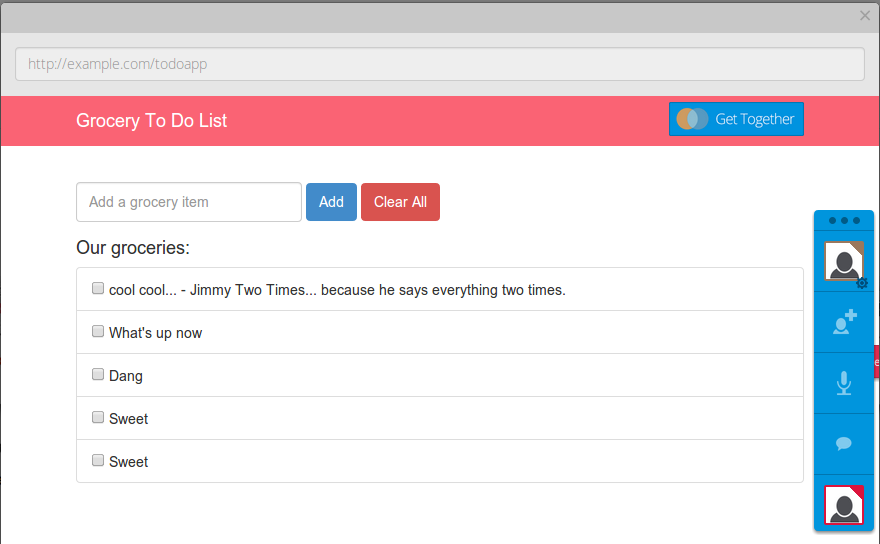
\includegraphics[scale=0.5]{img/togetherjs.png}
    \caption{Together.js}
\end{figure}

\begin{itemize}
\item
  Documentos são públicos para leitura, podendo também ser públicos para
  escrita se assim o usuário desejar.
\item
  Documentos são escritos em markdown com suporte a fórmulas matemáticas
  em LaTeX usando pandoc, MathJax.
\end{itemize}
\url{http://daringfireball.net/projects/markdown/dingus}: markdown é uma
linguagem de marcação fácil de ler e escrever que pode gerar textos
HTML, LaTeX.

\begin{figure}
    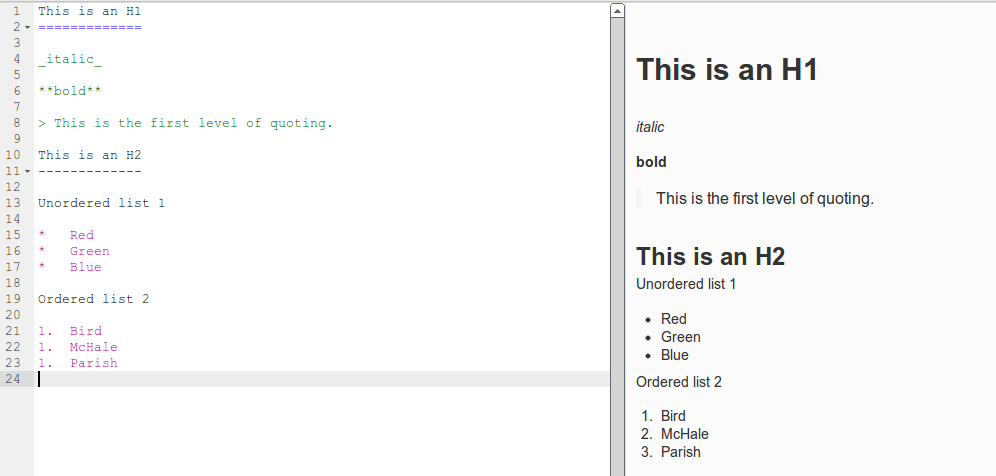
\includegraphics[scale=0.45]{img/markdown.png}
    \caption{Sintaxe Markdown}
\end{figure}

\url{http://johnmacfarlane.net/pandoc/}: converte textos em markdown
para HTML, LaTeX, entre outros.

\url{http://www.mathjax.org/}: renderiza fórmulas matemáticas LaTeX no
browser.

\begin{itemize}
\item
  Documentos podem ser exportados para PDF ou HTML usando pandoc.
\item
  Lista de links de referência.
\item
  Importar/Exportar de um arquivo markdown.
\item
  Documentos tem suporte a linguagens de programação, podendo o código
  ser embutido e mostrado com o devido highlighting.
\item
  Documentos podem ser apresentações em LaTeX beamer ou slides em HTML5.
\end{itemize}
\section{Objetivos}

\begin{itemize}
\item
  Proporcionar um local central de informações compartilhadas
\item
  Descentralizar a resolução de exercícios
\item
  Criar um local especializado na geração de documentos científicos
\item
  Incentivar alunos a utilizarem LaTeX desde cedo
\item
  Incentivar uso de tecnologias como markdown na criação de documentos
\item
  Aumentar o nível dos projetos haja vista que o número de projetos
  diferentes deverá aumentar.
\end{itemize}
\section{Tecnologias Utilizadas}

\begin{itemize}
\item
  Zend Framework 2 - ambiente web estável e completo.
\item
  Together.js - torna página colaborativa.
\item
  Mathjax - mostra fórmulas matemáticas escritas em LaTeX na web.
\item
  Pandoc - converte arquivos markdown em pdf, html.
\item
  Twitter Bootstrap 3 - front-end.
\item
  jQuery 2 - eventos, ajax.
\item
  Codemirror - web text editor.
\item
  FontAwesome 4 - icon web fonts.
\end{itemize}
